\documentclass[sigconf,screen,review]{acmart}
\usepackage{booktabs}
\usepackage{tikz}
\usetikzlibrary{positioning,arrows.meta}
\setcopyright{none}
\emergencystretch=1em
\settopmatter{printacmref=false}
\acmConference[WWW Companion '27]{Companion Proceedings of the ACM Web Conference 2027}{May 2027}{Dublin, Ireland}
\acmYear{2027}
\acmDOI{}
\acmISBN{}

\begin{document}
\title{OpenRec: Bridging Offline Experiments and Interactive Web Recommendation}
\author{Zheng Ma}
\affiliation{\institution{Alibaba}\city{Hangzhou}\country{China}}
\email{xsank@foxmail.com}
\renewcommand{\shortauthors}{Zheng Ma}

\begin{abstract}
A Web recommender combines candidate retrieval, feature computation, ranking, presentation rules, and user feedback. Studying these components only through offline model metrics leaves their interaction with a running application difficult to inspect. OpenRec is an open-source system connecting offline recommendation development to an interactive Web application. It combines configurable retrieval and ranking graphs, shared feature definitions with persisted fitted encoders, and feedback ingestion into serving state and historical data. The demonstration lets participants inspect candidate supply and result composition, connect a trained model's feature selection to online scoring, and observe how explicit feedback affects subsequent requests. A management console supports these activities through validated configuration and artifact changes. We describe the implemented recommendation paths, existing cross-component and offline evidence, and a hands-on session using example identities. Runtime interface captures illustrate the interaction, and KuaiRand experiments provide offline evidence for the shared feature representation.
\end{abstract}

\begin{CCSXML}
<ccs2012><concept><concept_id>10002951.10003317.10003347.10003350</concept_id><concept_desc>Information systems~Recommender systems</concept_desc><concept_significance>500</concept_significance></concept></ccs2012>
\end{CCSXML}
\ccsdesc[500]{Information systems~Recommender systems}
\keywords{recommender systems, Web applications, multi-stage recommendation, training-serving consistency, user feedback}
\maketitle

\section{Introduction}
Offline recommendation experiments produce retrieval scores or rankers; a Web application must also combine channels, filter exposed or disliked items, encode current features, and arrange a list. Feedback then changes later requests and supplies future training data. Model metrics alone cannot show which channels supplied candidates, whether scoring used the fitted representation, or when feedback reached serving state.

OpenRec connects these steps for researchers and developers. A Web page exposes recommendations, scores, and feedback; a console exposes graphs, feature selections, and evaluated artifacts. The 0.1.0 distribution pins compatible component revisions.\footnote{Project: \url{https://github.com/open-rec}.} Its three integrated capabilities are \emph{composable recommendation} across retrieval, ranking, and list policies; \emph{shared feature contracts} linking temporal samples and fitted encoders to serving; and \emph{observable feedback paths} into subsequent requests and training history. We contribute an implemented integration and demonstration, not a new ranker or a measured productivity gain.

\paragraph{Positioning.}
RecBole focuses on standardized recommendation model implementation and evaluation~\cite{recbole}; the earlier OpenRec framework emphasizes reusable algorithm modules~\cite{openrec2018}. Our project under the \texttt{open-rec} organization is distinct from that framework. The WWW demonstration RecAI organizes LLM-based recommendation tools around application capabilities~\cite{recai}. Our focus is the connection between offline artifacts and multi-stage, feedback-aware Web recommendation. Model publication is one supporting operation within this workflow; the demonstration also exposes recommendation-specific candidate supply, list policies, feature semantics, and feedback consumption.

\section{Connecting Experiments to Web Recommendation}
Figure~\ref{fig:architecture} adapts the project's Cluster architecture into online, streaming, offline, control, and monitoring paths. Figure~\ref{fig:item-graph} expands the default item DAG using its actual configuration. The full demonstration uses cluster mode; standalone supports smaller graph experiments and normally bypasses remote ranking.

\begin{figure*}[t]
\begin{minipage}[t]{0.49\textwidth}
\centering
% Paper adaptation of .github/profile/README.md: Cluster architecture.
% Group storage/compute roles and show selected API/data/control links.
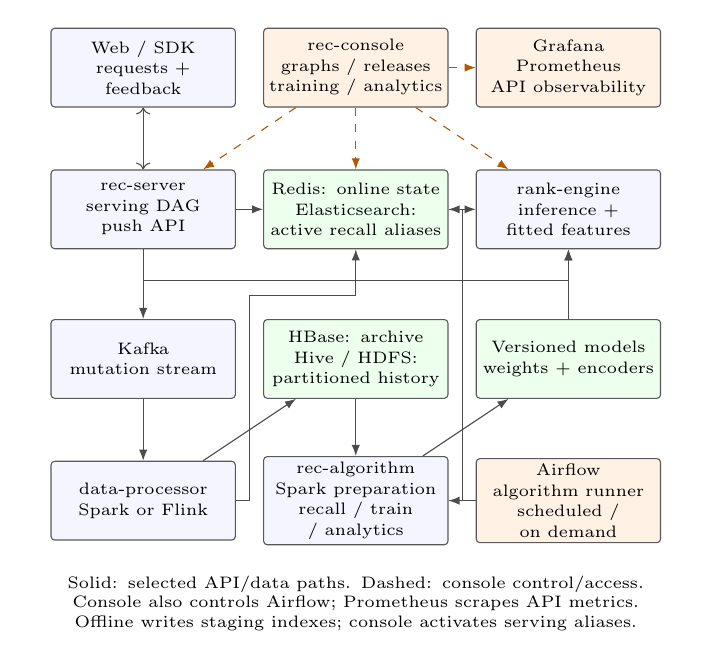
\begin{tikzpicture}[x=1mm,y=1mm,font=\fontsize{6.5}{7.4}\selectfont,
 box/.style={draw=black!65,rounded corners=1.3pt,align=center,text width=22mm,minimum height=10mm,inner sep=2pt,fill=blue!4},
 store/.style={box,fill=green!7},
 ctrl/.style={box,fill=orange!10},
 data/.style={-{Latex[length=1.4mm]},draw=black!70},
 ctl/.style={data,dashed,draw=orange!70!black}]
\node[box] (client) at (0,0) {Web / SDK\\requests + feedback};
\node[ctrl] (console) at (27,0) {rec-console\\graphs / releases\\training / analytics};
\node[ctrl] (metrics) at (54,0) {Grafana\\Prometheus\\API observability};
\node[box] (server) at (0,-18) {rec-server\\serving DAG\\push API};
\node[store] (serving) at (27,-18) {Redis: online state\\Elasticsearch:\\active recall aliases};
\node[box] (rank) at (54,-18) {rank-engine\\inference +\\fitted features};
\node[box] (kafka) at (0,-37) {Kafka\\mutation stream};
\node[store] (history) at (27,-37) {HBase: archive\\Hive / HDFS:\\partitioned history};
\node[store] (models) at (54,-37) {Versioned models\\weights + encoders};
\node[box] (processor) at (0,-55) {data-processor\\Spark or Flink};
\node[box] (offline) at (27,-55) {rec-algorithm\\Spark preparation\\recall / train / analytics};
\node[ctrl] (airflow) at (54,-55) {Airflow\\algorithm runner\\scheduled / on demand};
\draw[data,<->] (client)--(server);
\draw[ctl] (console)--(server);
\draw[ctl] (console)--(serving);
\draw[ctl] (console)--(rank);
\draw[ctl] (console)--(metrics);
\draw[data] (server)--(serving);
\draw[data] (server.south) -- (0,-27) -- (54,-27) -- (rank.south);
\draw[data] (server)--(kafka);
\draw[data] (kafka)--(processor);
\draw[data] (processor)--(history);
\draw[data] (processor.east) -- (13.5,-55) -- (13.5,-29) -- (27,-29) -- (serving.south);
\draw[data] (history)--(offline);
\draw[data] (airflow)--(offline);
\draw[data] (offline)--(models);
\draw[data] (models)--(rank);
\draw[data] (serving)--(rank);
\draw[data] (offline.east) -- (40.5,-55) -- (40.5,-18) -- (serving.east);
\node[align=center,font=\fontsize{6}{7}\selectfont,text width=81mm] at (27,-68)
 {Solid: selected API/data paths. Dashed: console control/access.\\Console also controls Airflow; Prometheus scrapes API metrics.\\Offline writes staging indexes; console activates serving aliases.};
\end{tikzpicture}

\caption{Cluster architecture adapted from the project profile: online serving, feedback, offline computation, control, analytics, and monitoring. Console publication connects staged artifacts to serving.}
\label{fig:architecture}
\Description{Cluster components: Web and SDK, rec-server, Redis and Elasticsearch, rank-engine, Kafka, Spark or Flink processing, HBase and Hive history, offline algorithms, model artifacts, Airflow, console and monitoring.}
\end{minipage}\hfill
\begin{minipage}[t]{0.49\textwidth}
\centering
% All 17 configured nodes and 18 edges, with exact dependency groups.
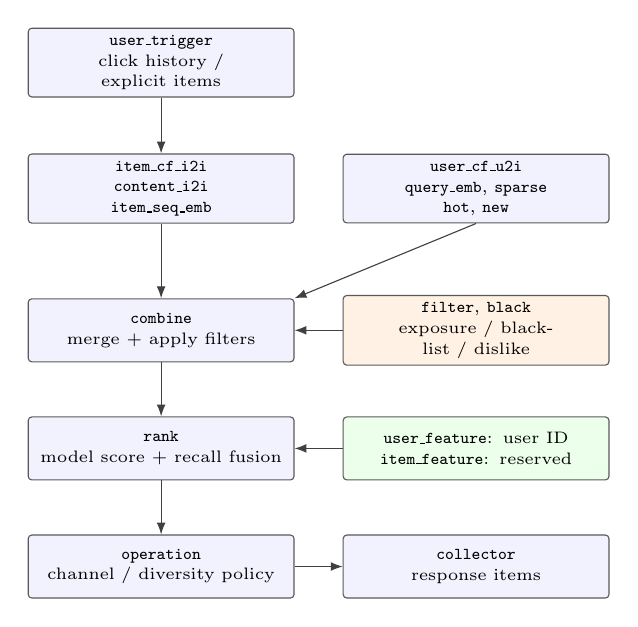
\begin{tikzpicture}[x=1mm,y=1mm,font=\fontsize{6.5}{7.5}\selectfont,
 box/.style={draw=black!65,rounded corners=1.3pt,align=center,text width=32mm,minimum height=8mm,inner sep=2.5pt,fill=blue!5},
 dep/.style={-{Latex[length=1.5mm]},draw=black!75}]
\node[box] (trigger) at (0,0) {\texttt{user\_trigger}\\click history / explicit items};
\node[box] (triggered) at (0,-16) {\texttt{item\_cf\_i2i}\\\texttt{content\_i2i}\\\texttt{item\_seq\_emb}};
\node[box] (independent) at (40,-16) {\texttt{user\_cf\_u2i}\\\texttt{query\_emb}, \texttt{sparse}\\\texttt{hot}, \texttt{new}};
\node[box] (combine) at (0,-34) {\texttt{combine}\\merge + apply filters};
\node[box,fill=orange!10] (filters) at (40,-34) {\texttt{filter}, \texttt{black}\\exposure / blacklist / dislike};
\node[box] (rank) at (0,-49) {\texttt{rank}\\model score + recall fusion};
\node[box,fill=green!8] (features) at (40,-49) {\texttt{user\_feature}: user ID\\\texttt{item\_feature}: reserved};
\node[box] (operation) at (0,-64) {\texttt{operation}\\channel / diversity policy};
\node[box] (collector) at (40,-64) {\texttt{collector}\\response items};
\draw[dep] (trigger)--(triggered);
\draw[dep] (triggered)--(combine);
\draw[dep] (independent.south) -- (combine.north east);
\draw[dep] (filters)--(combine);
\draw[dep] (combine)--(rank);
\draw[dep] (features)--(rank);
\draw[dep] (rank)--(operation);
\draw[dep] (operation)--(collector);
\end{tikzpicture}

\caption{Configured item DAG: 17 nodes, 18 dependencies. Arrows apply to every named node in a group. User-feature supplies the user ID; item-feature is a reserved hook. Actual encoding runs in rank-engine.}
\label{fig:item-graph}
\Description{Click or explicit-item triggers feed three recall nodes. Five other recall nodes and two filter nodes feed combine. Combine, the user-ID node, and a reserved item-feature hook precede rank, followed by operation and collector.}
\end{minipage}

\end{figure*}

\begin{figure*}[t]
\centering
\begin{minipage}[t]{0.55\textwidth}
\centering\small\textbf{(A) Recommendation and feedback}\\[1mm]
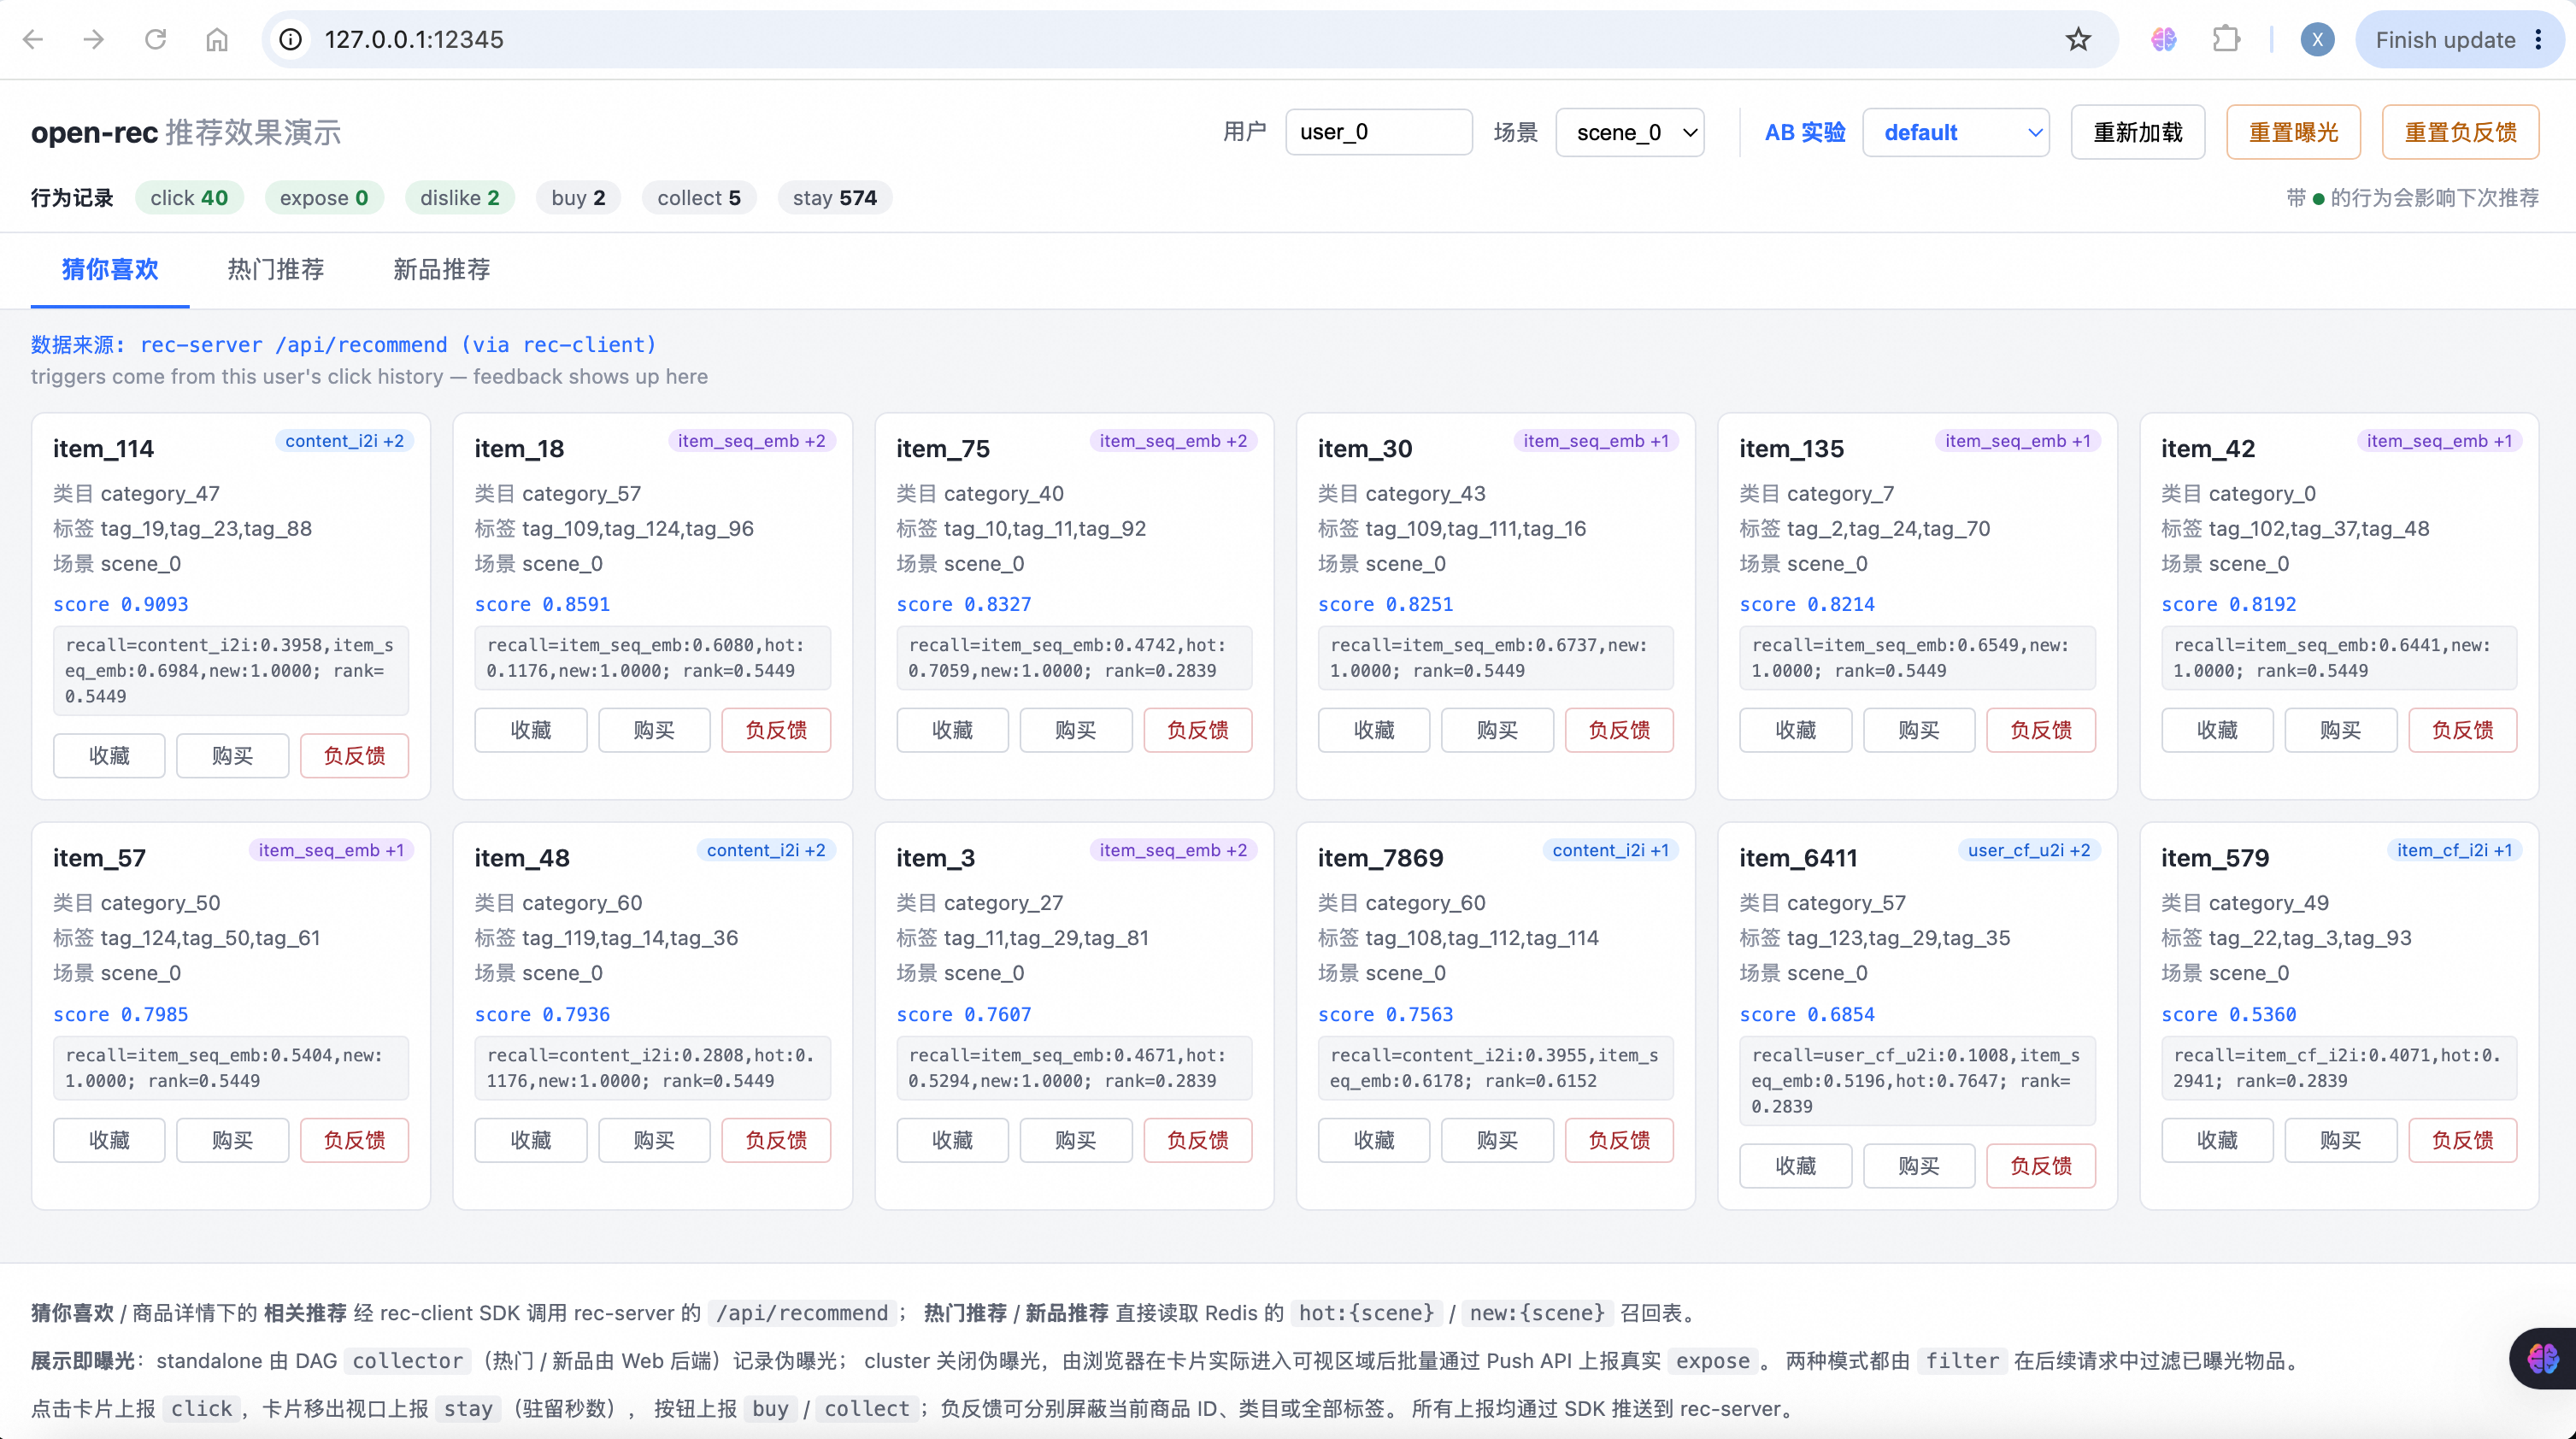
\includegraphics[height=37mm,trim=35bp 748bp 2509bp 480bp,clip]{figures/openrec_rec_items.png}\\[3mm]
\textbf{(C) User and candidate feature selection}\\[1mm]
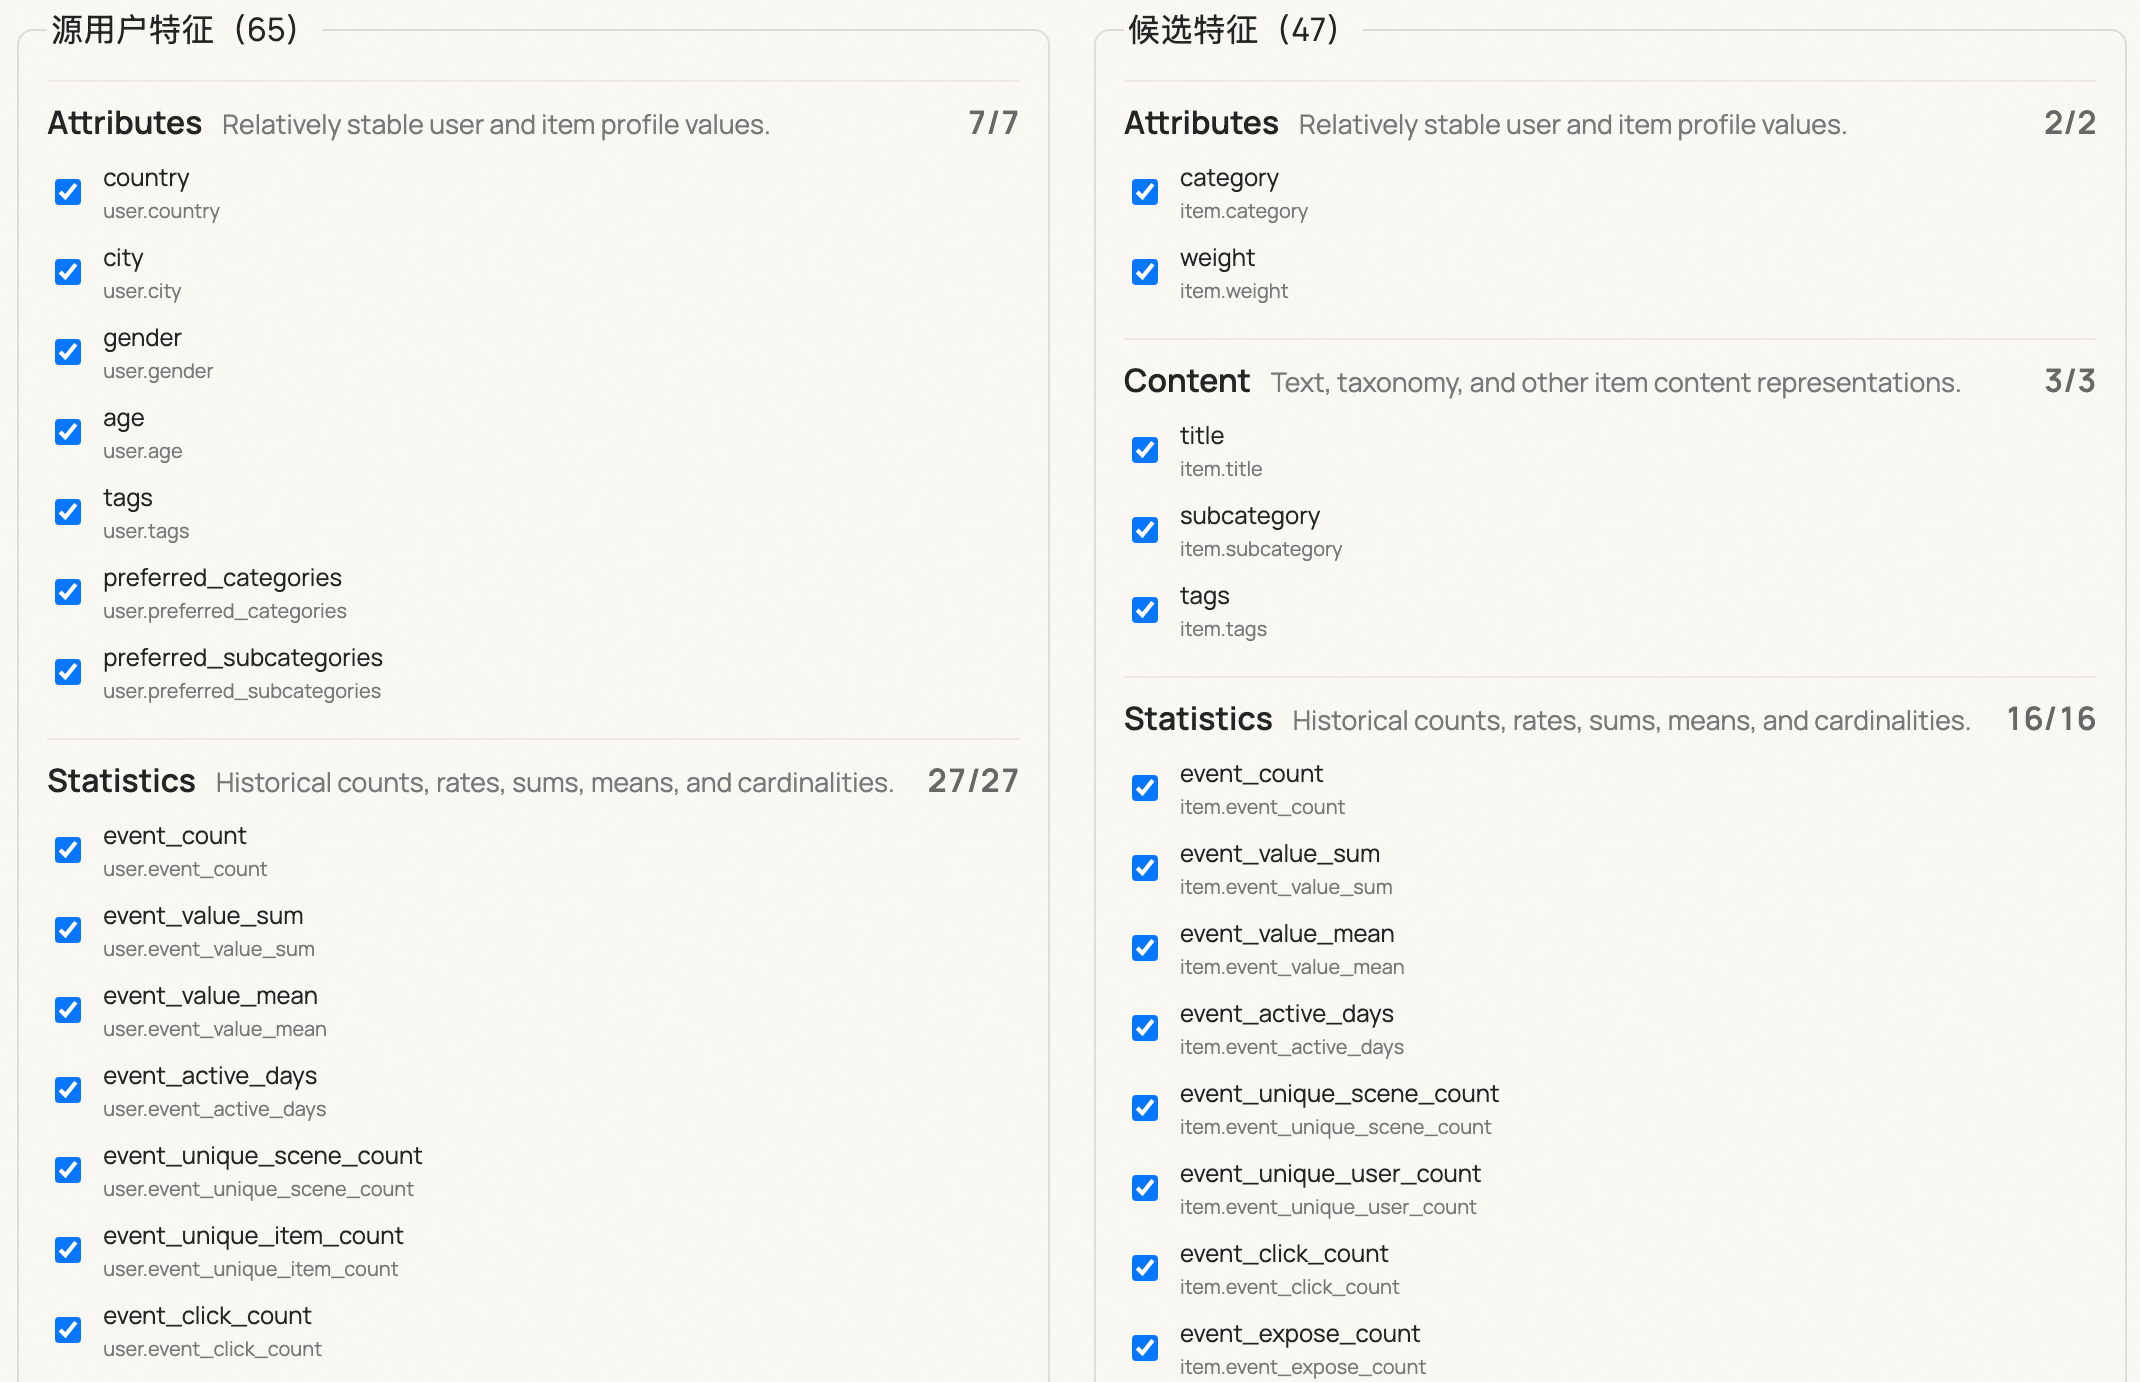
\includegraphics[width=\linewidth]{figures/openrec_feature.png}
\end{minipage}\hfill
\begin{minipage}[t]{0.42\textwidth}
\centering\small\textbf{(B) Operation policy configuration}\\[1mm]
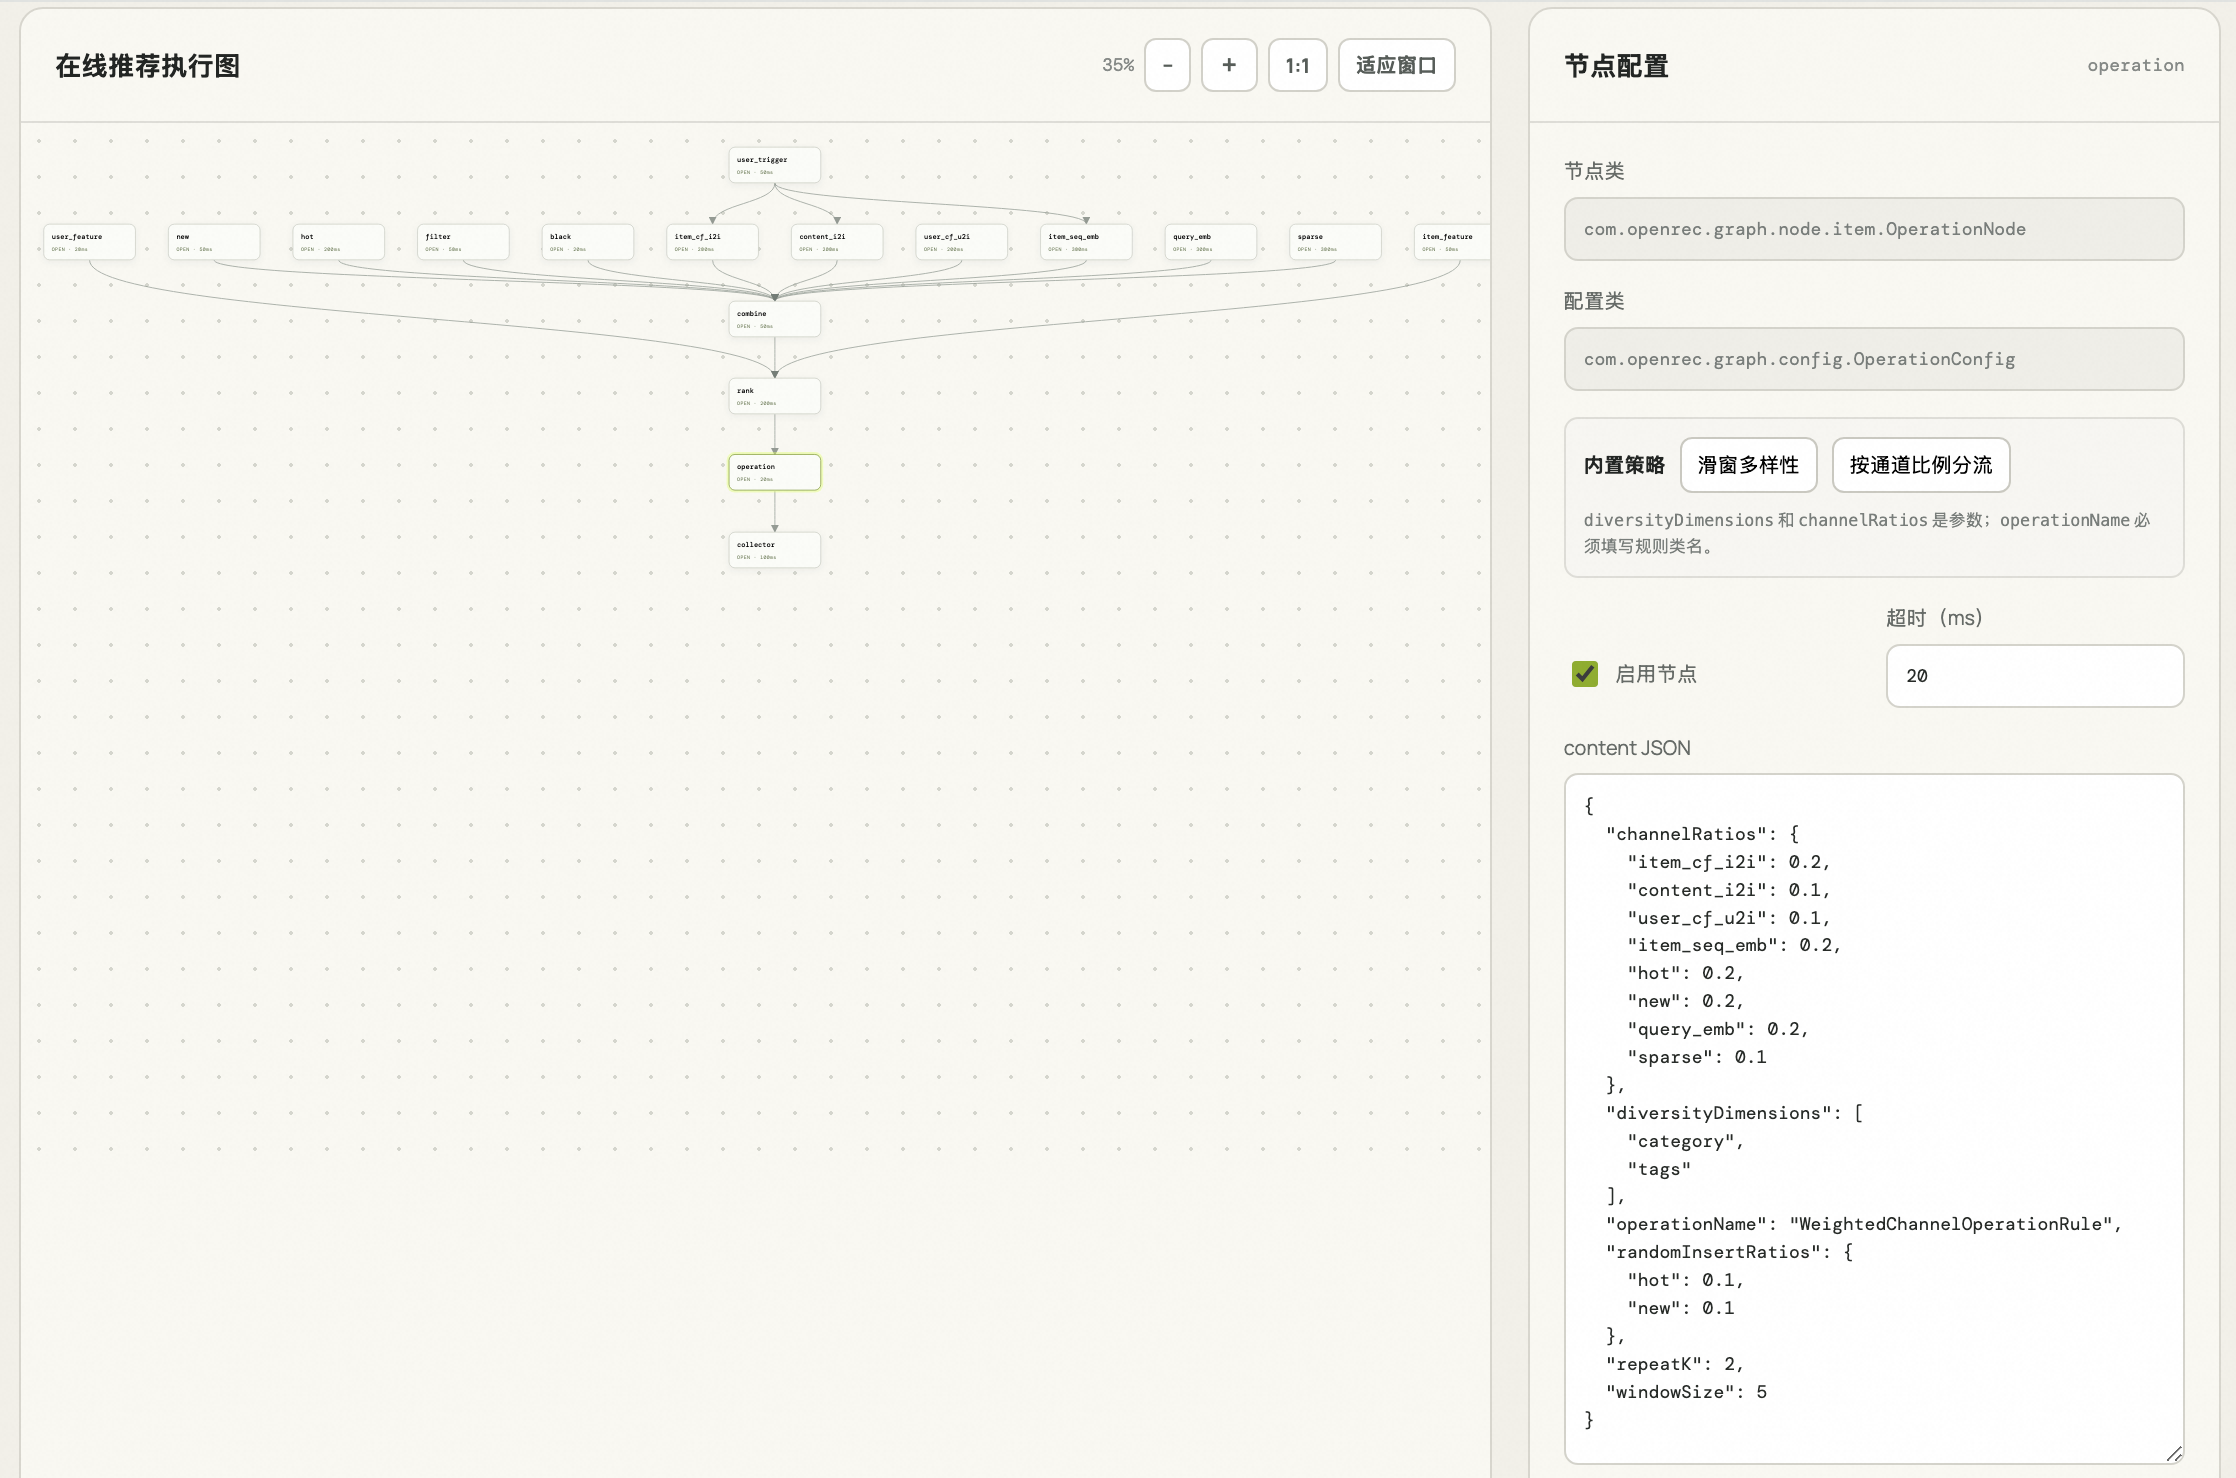
\includegraphics[width=\linewidth,trim=1550bp 8bp 25bp 415bp,clip]{figures/openrec_node_config.png}
\end{minipage}
\caption{Runtime captures: (A) recommendation scores and feedback (user\_0, scene\_0, default); (B) operation presets and parameters, with channel allocation selected; (C) user/candidate feature selection by attribute, content, and statistics groups. The training form does not establish a completed run or loaded model.}
\label{fig:runtime}
\Description{Actual recommendation card, operation policy presets and configuration JSON, and the complete supplied feature-selection capture with both user and candidate columns. English panel headings accompany the original interface.}
\end{figure*}

\subsection{Candidate Supply and Result Composition}
Figure~\ref{fig:item-graph} expands the item-serving DAG inside rec-server. Eight retrieval channels feed candidate combination alongside exposure and blacklist inputs; the user-ID and reserved feature nodes precede ranking, followed by a list policy and collection. With \texttt{debug=true}, the API reports recall-node status and output counts before filtering and final selection. Result cards show channel labels and distinguish recall from rank scores. These views separate candidate supply from final list membership: an overlapping candidate can be retrieved by several channels but occupy only one result slot.

Beyond enabling channels, developers can configure recall/rank score fusion and post-ranking policies. A channel-allocation rule divides result slots by normalized channel ratios, assigning overlapping candidates to their primary channel and filling shortages by score. An alternative sliding-window rule limits repeated category or tag attributes. Strict constraints can yield fewer results if the candidate pool is insufficient. These are configurable list policies, not guarantees of improved relevance.

Graph changes apply to named experiments selected through \texttt{params.ab}. Validation checks supported nodes, typed configuration, and dependencies; requests retain their selected graph snapshot. Readiness probes verify representative execution after publication. The console retains versions for restoration. Neither statistical A/B analysis nor candidate-level causal explanations are provided.

\subsection{From Feature Definitions to Online Scores}
OpenRec separates four artifacts: canonical logical feature definitions, a model's ordered feature selection, fitted encoders, and materialized feature values. The catalog describes semantics such as event identity, aggregation windows, time boundaries, and online/offline availability. Offline pandas/Spark implementations and the streaming feature core implement these contracts; shared fixtures check selected behaviors across implementations. Cluster training prepares point-in-time samples from mutation history so that later events and entity updates are not simply joined into earlier labels.

The console offers supported LR, FM, and LightGBM feature selections and triggers offline training through Airflow. Training produces evaluated releases; it does not update the live model. Each release binds weights to selected feature definitions, fitted vocabularies/scaling, input dimensions, and checksums. The ranking service imports the algorithm library's encoding contracts and loads the retained fitted representation instead of fitting a new encoder on serving data. It checks selected definitions and materialized columns before activation and uses a consistent model/feature snapshot for a score request.

Deployment supports a narrower feature subset than the research code. Catalog membership does not establish complete or fresh online values. Cache refresh is separate from stream updates; failures retain the previous snapshot. New features require implementation, historical preparation, and deployment verification.

\subsection{Feedback into Serving and Future Training}
The Web application reports visible-card exposures, clicks, and structured dislikes through the ingestion API. In cluster mode, Kafka carries events to a Flink or Spark processor, which updates Redis projections and retains history for offline computation. Recent clicks supply retrieval triggers; exposure history and dislike rules support filtering. A dislike can target an item, category, or tags. Behavioral aggregates update user and item feature snapshots; the ranking service must refresh its encoded cache before those updates can affect model inputs.

Retained history supports future recall computation and training. Jobs stage indexes; the console validates and activates serving aliases. Retraining and publication are explicit, not immediate online learning. Graph, recall, and model lifecycles are separate; restoring one does not rewind feedback or the whole system.

\section{Interactive Demonstration}
The demonstration uses OpenRec's existing cluster deployment, launched with the distribution's \texttt{example\_cluster/start.sh}. This mode connects the recommendation application and management console to online ranking, streaming feedback processing, and offline jobs. A cluster instance is already running; Figure~\ref{fig:runtime} shows captures from the existing interfaces. Participants use an example identity to browse recommendations, inspect the serving configuration, and submit feedback. The following walkthrough connects these interactions to the three system capabilities.

\subsection{Explore Candidate Supply and List Policies}
The recommendation page displays items, channel labels, recall/rank scores, and feedback controls (Figure~\ref{fig:runtime}A). The presenter opens the corresponding serving graph in the console and explains how retrieval channels, filters, ranking, and list policies compose the response. Participants can inspect node configuration and compare the channel-allocation and diversity presets (Figure~\ref{fig:runtime}B).

To illustrate a configuration change, the presenter disables a contributing recall channel in a named experiment, publishes the graph, and requests recommendations using that experiment. Debug output exposes the channel's execution status and candidate count. The final list may remain unchanged when other channels retrieve the same items. With the operation plugin loaded, participants can also compare result-channel composition, repeated attributes, and list length under different policies. This illustrates configurable behavior rather than a controlled relevance comparison.

\subsection{Connect Selected Features to Scoring}
The console's training configuration groups user and candidate features by attributes, content, and statistics (Figure~\ref{fig:runtime}C). The presenter connects a prepared model release to its selected features, fitted encoding sidecar, input dimension, and offline evaluation. The model-management view and ranking-service state identify the active release; scores on the recommendation page show its use in the serving path.

Participants can inspect these artifacts without running a training job during the session. The presenter can additionally demonstrate activation and restoration of prepared compatible releases. Changing a trained model's feature selection requires retraining; merely editing the training form does not alter the active ranker.

\subsection{Follow Feedback into Subsequent Requests}
Participants submit clicks or dislikes through the recommendation page. The presenter traces feedback through the cluster's streaming path: recent clicks can supply retrieval triggers, while projected dislike rules are consumed by filtering on subsequent requests. An item-level dislike illustrates the distinction between accepting an event and applying its effect after asynchronous projection.

The presenter uses diagnostics to inspect the projected rule and the active filter configuration, alongside the refreshed recommendation list. List disappearance alone does not identify its cause, since exposure filters and other policies also affect membership. Feature updates and ranking-cache refresh are separate steps; feedback does not imply immediate retraining or a guaranteed score change.

\paragraph{On-site deployment.}
The conference demonstration will use this cluster mode on a prepared host, with browser access to the recommendation page and console. Data, recall indexes, and compatible model releases will be loaded before the session. The presenter will guide configuration changes, restore graph/model versions between sessions, and use separate example identities for feedback interactions. English annotations and a guided walkthrough will accompany the primarily Chinese interface.

\section{Evaluation}
\paragraph{Dataset and protocol.}
We evaluate click prediction using OpenRec's shared point-in-time (PIT) features on KuaiRand-1K~\cite{kuairand,experiments}. Labels use \texttt{is\_click}; standard and random-policy test subsets follow \texttt{is\_rand}. LR, FM, and LightGBM use the same temporal split and 33 logical features: 16 user behavioral statistics, 16 item behavioral statistics, and one scene feature, yielding 46 encoded inputs. The selected catalog features support both online and offline computation. Each learned model is evaluated with seeds 42, 43, and 44. Random-policy observations are excluded from training, validation selection, and feature history; evaluation features are frozen at the training boundary with a one-hour feedback delay. LightGBM uses a binary objective for independent exposure rows.

\begin{table}[t]
\caption{KuaiRand-1K temporal holdout results. Learned-model entries are means over three seeds; popularity is deterministic. Full per-run metrics and sample standard deviations are available in the experiment report~\cite{experiments}.}
\label{tab:kuairand}
\centering\small
\begin{tabular}{@{}lrrr@{}}
\toprule
& Standard & \multicolumn{2}{c}{Random policy}\\
\cmidrule(l){2-2}\cmidrule(l){3-4}
Model & AUC $\uparrow$ & AUC $\uparrow$ & LogLoss $\downarrow$\\
\midrule
Popularity & 0.52956 & 0.52949 & \textbf{0.57823}\\
LR + PIT & 0.75142 & 0.66737 & 0.68590\\
FM + PIT & 0.75169 & 0.67316 & 0.69849\\
LightGBM + PIT & \textbf{0.75410} & \textbf{0.67690} & 0.71215\\
\bottomrule
\end{tabular}
\end{table}

\paragraph{Results and interpretation.}
Table~\ref{tab:kuairand} compares the three rankers with a popularity baseline. LightGBM achieves the highest AUC under both evaluation policies, while popularity has the lowest random-policy LogLoss. Thus, higher AUC does not imply lower probabilistic prediction loss. The random-policy AUC sample standard deviations are 0.00036, 0.00113, and 0.00079 for LR, FM, and LightGBM, respectively. Compared with the earlier behavior-only configuration in the report, the shared PIT selection increases random-policy AUC by 0.00361 for LR and 0.01393 for FM. These results support the use of shared temporal features and offer concrete model tradeoffs for the scoring demonstration. They do not establish online uplift or verify that an experimental checkpoint and its feature values have been deployed in the demonstration environment.

\paragraph{System verification.}
The 0.1.0 validation record documents component tests, feature/SDK contract checks, a real-Elasticsearch lifecycle test, and local cluster runs covering ranked requests and streaming checks~\cite{release}. These complement the offline results by checking integration behavior. Figure~\ref{fig:runtime} illustrates the running interfaces, while the three demonstration tasks specify observable channel, model, and feedback behavior. We make no end-to-end latency or throughput claim.

\balance
\section{Ethical Use and Availability}
We use example identities and fixture data, without collecting personal profiles or conducting a user study. Offline research data retain their providers' access and licensing restrictions and are not redistributed. Captures exclude credentials and sensitive identifiers. Because the console lacks authentication and role-based access control, the venue deployment will be isolated and presenter-supervised.

\section{Conclusion}
OpenRec connects offline recommendation development to Web serving through composable pipelines, shared feature contracts, and feedback processing. The demonstration exposes these connections through candidate supply, list policies, model inputs, and subsequent requests, with explicit publication and bounded restoration.

\bibliographystyle{ACM-Reference-Format}
\bibliography{references}
\end{document}
